%%%%%%%%%%%%%%%%%%%%%%%%%%%%%%%%%%%%%%%%%%%%%%%%%%%%%%%%%%%
%
% Using the same LaTeX template as Brooke Simmons HST Proposal.
% This is used in HST applications with STScI.
% PHASE I: Archival & Theoretical Research Proposal Template
%
% I'm open to changing the proposal template.

\documentclass[11pt]{article}
\usepackage{phase1}
\usepackage{wrapfig}
\usepackage{caption}
\usepackage{multicol}
\usepackage{graphicx, graphics}
\usepackage{enumitem}
\usepackage[utf8]{inputenc}
\usepackage[T1]{fontenc}
\usepackage{natbib}
\usepackage{hyperref}
\usepackage{ae,aecompl}
\usepackage{color}

\title{ESA Fellowship Proposal: Statistically Constraining the Interacting Galaxy Population}
\author{David O'Ryan}

\definecolor{titlecol1}{rgb}{0.7,0.0,0.05} %dark red
\definecolor{titlecol2}{rgb}{0.039,0.361,0.569} %teal++

\begin{document}
    \begin{center}
        \large{{Proposal: Towards a Statistical Understanding of Galaxy Evolution \\
        Potential Fellow: David O'Ryan \\
        Potential Mentor(s): Bruno Alteiri \& Bruno Merin}}
    \end{center}
    
% \vspace{-7mm}
% \begin{abstract}
% \vspace{-3.5mm}
% Relating the fundamental parameters of galaxies to a multitude of underlying processes and their morphology is a notoriously difficult task. Often, data containing fully parameterised galaxies is sparse (or concentrated in specific areas of the sky) while morphological classification data of galaxies is limited. Rarely do these sets of data overlap. The result of this is that we have a complete disconnect between investigating the morphological relationship of galaxies with their parameterisation. By using the newly released convolutional network \texttt{Zoobot} from the Galaxy Zoo collaboration and the recently launched Euclid observatory, I will rectify this. I will create the largest catalogue of morphologically classified galaxies with complete ancillary data to date. This catalogue will be similar to the COSMOS catalogue, but across the entire sky. We will conduct initial analysis of this catalogue before releasing it to the community for further use. We will conduct initial analysis of this catalogue, linking a multitude of parameters with morphology, and inferring links between underlying physical processes within galaxies to their parameters and morphology. We will also conduct in depth analysis of a specific galaxy type in this catalogue to show its power: interacting galaxies. 
% \end{abstract}

\vspace{-5mm}
\justification
\vspace{-3mm}
\noindent\textbf{Galaxy Morphology, Photometric Parameterisation and Galaxy Evolution} \\
Galaxy morphology is a key indicator of galactic evolutionary history. Whether a galaxy is elliptical or a disk, is barred or unbarred, is spiral or elliptical, we can immediately form some base assumptions about it. As some examples, spiral galaxies are often gas rich and star forming when compared to often gas poor and quiescent elliptical galaxies \citep{2022MNRAS.510.4126S}, evidence is growing that strongly barred galaxies are more likely to have active nuclear regions than their weakly barred or non-barred counterparts \citep{izzy..paper} and disk-dominated galaxies are likely to have a merger-free history \citep{2017MNRAS.470.1559S}. To fully understand the link between morphology and a galaxies evolutionary history we need large catalogues of morphologically classified galaxies. A current example of these catalogues are created by volunteers and citizen scientists visually inspecting galaxy images in the Galaxy Zoo collaboration \cite{2008MNRAS.389.1179L}. However, the time constraints of visually inspecting sources means the size of such catalogues is often limited. Once we start to control these catalogues for various morphologies, we often find that our samples cannot hold statistical significance.

A recent development in morphology classification has been the accuracy and efficiency of a new model: \texttt{Zoobot} \cite{2023JOSS....8.5312W}. It is a convolutional neural network (CNN) trained to answer all thirty four classification tasks in the Galaxy Zoo workflow. It has had significant success in a number of works, from finding interacting galaxies in the \textit{Hubble Space Telescope} (HST) archives \cite{2023ApJ...948...40O}, to successfully matching the volunteer responses to 314,000 galaxies in the Galaxy Zoo DECaLS project \cite{2022MNRAS.509.3966W}, to successfully classifying the morphology of 8.7 million galaxies in the Galaxy Zoo: DESI project \cite{mikes..paper}. Thus, providing large sub-samples of different galaxy morphologies and pioneering insights into the interplay between morphology and the underlying physical processes driving galaxy evolution. 

Another set of classifications important to galaxy evolution is photometric parameterisation. These are parameters measured from a galaxy's emission lines using spectral energy distribution (SED) fitting. The resulting catalogues provide the stellar masses, star formation rates, nuclear activity and a host of other parameters. These SED matches are conducted with well used astrophysical softwares such as the Easy and Accurate zPhot from Yale (EAzY; \citet{2008ApJ...686.1503B}) and the Fitting and Assessment of Synthetic Templates (FAST; \citet{2009ApJ...700..221K}). Many examples of such ancillary catalogues have been produced, a prime example being the Cosmic Evolution Survey \citep[COSMOS; ][]{2007ApJS..172...99C} catalogue. These contain the parameterisations of over 1.8 million galaxies focused on a 3$^{\circ} \times $3$^{\circ}$ area of the sky. This catalogue has seen significant use by the community, with the initial data release having over 650 citations.

However, the size of catalogues which overlap morphological and ancillary data remains limited. Therefore, a key opportunity exists to enhance our understanding of the interplay between observable galactic morphology, their parameterisations and specific evolutionary processes. I will create a combined, statistically significant catalogue completely overlapping ancillary and morphological data which will be the largest to date. I will then conduct initial analysis to demonstrate its applicability. This will be achieved by combining the tried and tested CNN \texttt{Zoobot} with ESA Datalabs and utilising the incoming survey data of Euclid.

\vspace{-5mm}
\impact
\vspace{-3mm}
\noindent \textbf{Galaxy Evolution Over the Last 8 Billion Years} \\
\noindent Throughout my PhD, my research has been focused on the effects of interaction and merging on galaxy evolution. The specific influence of galaxy interaction, when two galaxies come close enough to have a gravitational effect upon one another, are poorly understood. In general, interaction leads to a sudden increase in star formation \citep{2021MNRAS.503.3113M} often causing quenching \citep{2023RAA....23b5016D}, severe morphological disturbance \citep{1972ApJ...178..623T} and is often linked to the ignition of nuclear activity \citep{2015ApJ...806..219C}. To explore the variations in these effects, and quantify their impact on evolution, we require large catalogues of interacting and merging galaxies to fully explore the underlying parameter space.

Creating these catalogues by visual inspection is a notoriously difficult task. Numerous works have shown that classifications from citizen scientists \citep{2010MNRAS.401.1552D} or machine learning \citep{2022A&A...661A..52P} techniques often lead to significant levels of contamination by close pairs. I.e., contamination from galaxies which appear close together in the two dimensional plane of the sky but are at very different redshifts. I have worked on numerous projects which are attempting to overcome this difficulty \citep{bertas..paper, 2022MNRAS.513.1459M} but my primary contribution was using \texttt{Zoobot} to build a pure catalogue. In \citet{2023ApJ...948...40O}, I used the \texttt{Zoobot} with ESA Datalabs to explore the HST archives for interacting galaxies. A total of 92 million sources were classified into interacting and non-interacting, creating a catalogue of 21,926 interacting galaxies. The largest to date. This was the first published work where \texttt{Zoobot} was used to such a scale on a specific classification problem. This initial use of \texttt{Zoobot} was described in the official release paper of the model \citep{2023JOSS....8.5312W}. 

An unintended result of using \texttt{Zoobot} in this way with ESA Datalabs was that a host of other objects of astrophysical interest were discovered in the archives. Because interacting galaxies are often morphologically disturbed and highly irregular, \texttt{Zoobot} misclassified many objects of morphological or astrophysical interest as interacting galaxies. As a byproduct of my approach, I therefore created some of the largest catalogues of various astrophysical objects to date. Examples of these extra objects include ring galaxies, overlapping galaxies, quasars and edge-on proto-planetary disks. The latter objects we only have three known examples of. This approach, and internship, gave me a unique insight into how to use ESA Datalabs to efficiently provides me with a large repository of existing pipelines to stream line the ramp up of this project.

Now that a large catalogue of interacting galaxies has been created, it is possible to explore their underlying parameters and attempt to make inferences into their interplay with morphology and parameterisations. One way I am investigating this is by using simulations. I have developed software to directly compare observations and simulations. This code mimics the methodology of \citet{2016MNRAS.459..720H}, a successful project constraining the stellar masses, orientations and sizes of interacting galaxies with citizen scientists.

Another approach I am adopting is to use ancillary data from different catalogues to find the underlying parameters of interaction. I have matched the \citet{2023ApJ...948...40O} catalogue to the COSMOS2020 \citep{2022ApJS..258...11W} catalogue and created a sample of 4,000 interacting galaxies (all galaxies which overlap between the catalogues) with parameterisation data readily available. This work remains in progress, but the relation between galaxy interaction, environment, nuclear activity, star formation enhancement and projected separation is being investigated. This work, which will be published before I begin this fellowship, and the pipelines being built will form the basis of the analysis work of this project.

\vspace{-3mm}
\describearchival
\vspace{-3mm}
This project has six key goals which will be achieved with four scientific results (R$N$) and two deliverables (D$N$). I have defined four \textbf{work packages} (WPs) that follow the full process of this project across eleven different tasks. For a full breakdown of the expected timeline, specific tasks and their WPs please see Figure \ref{fig:gantt-chart}. The project goals are:
\begin{enumerate}[itemsep=0pt, parsep=0pt, topsep=5pt]
    \item To create a fully open, and accessible image repository of every extended source at rest frame in the \textit{Hubble} and JWST public archives (T1.1; D1). 
    \item To apply \texttt{Zoobot} to the above created repository and gain morphological classifications of an unprecedented number of galaxies (T1.2, T1.3; R1).
    \item To utilise Euclid data to create a catalogue of ancillary data to the scale of the morphological catalogue. The size of this catalogue will also be unprecedented (T2.1, T2.2, T2.3; R2).
    \item To match these catalogues and create an advanced catalogue, while fully diagnosing their accuracy and completeness (T3.1, T3.2; R3).
    \item To create the largest catalogue of spectroscopically confirmed interacting galaxies to date (T4.1; D2).
    \item To analyse the advanced catalogues in relation to the interplay between galaxy interaction and the ignition of nuclear activity, demonstrating their use (T4.2, T4.3; R4).
\end{enumerate}

\begin{figure}
    \centering
    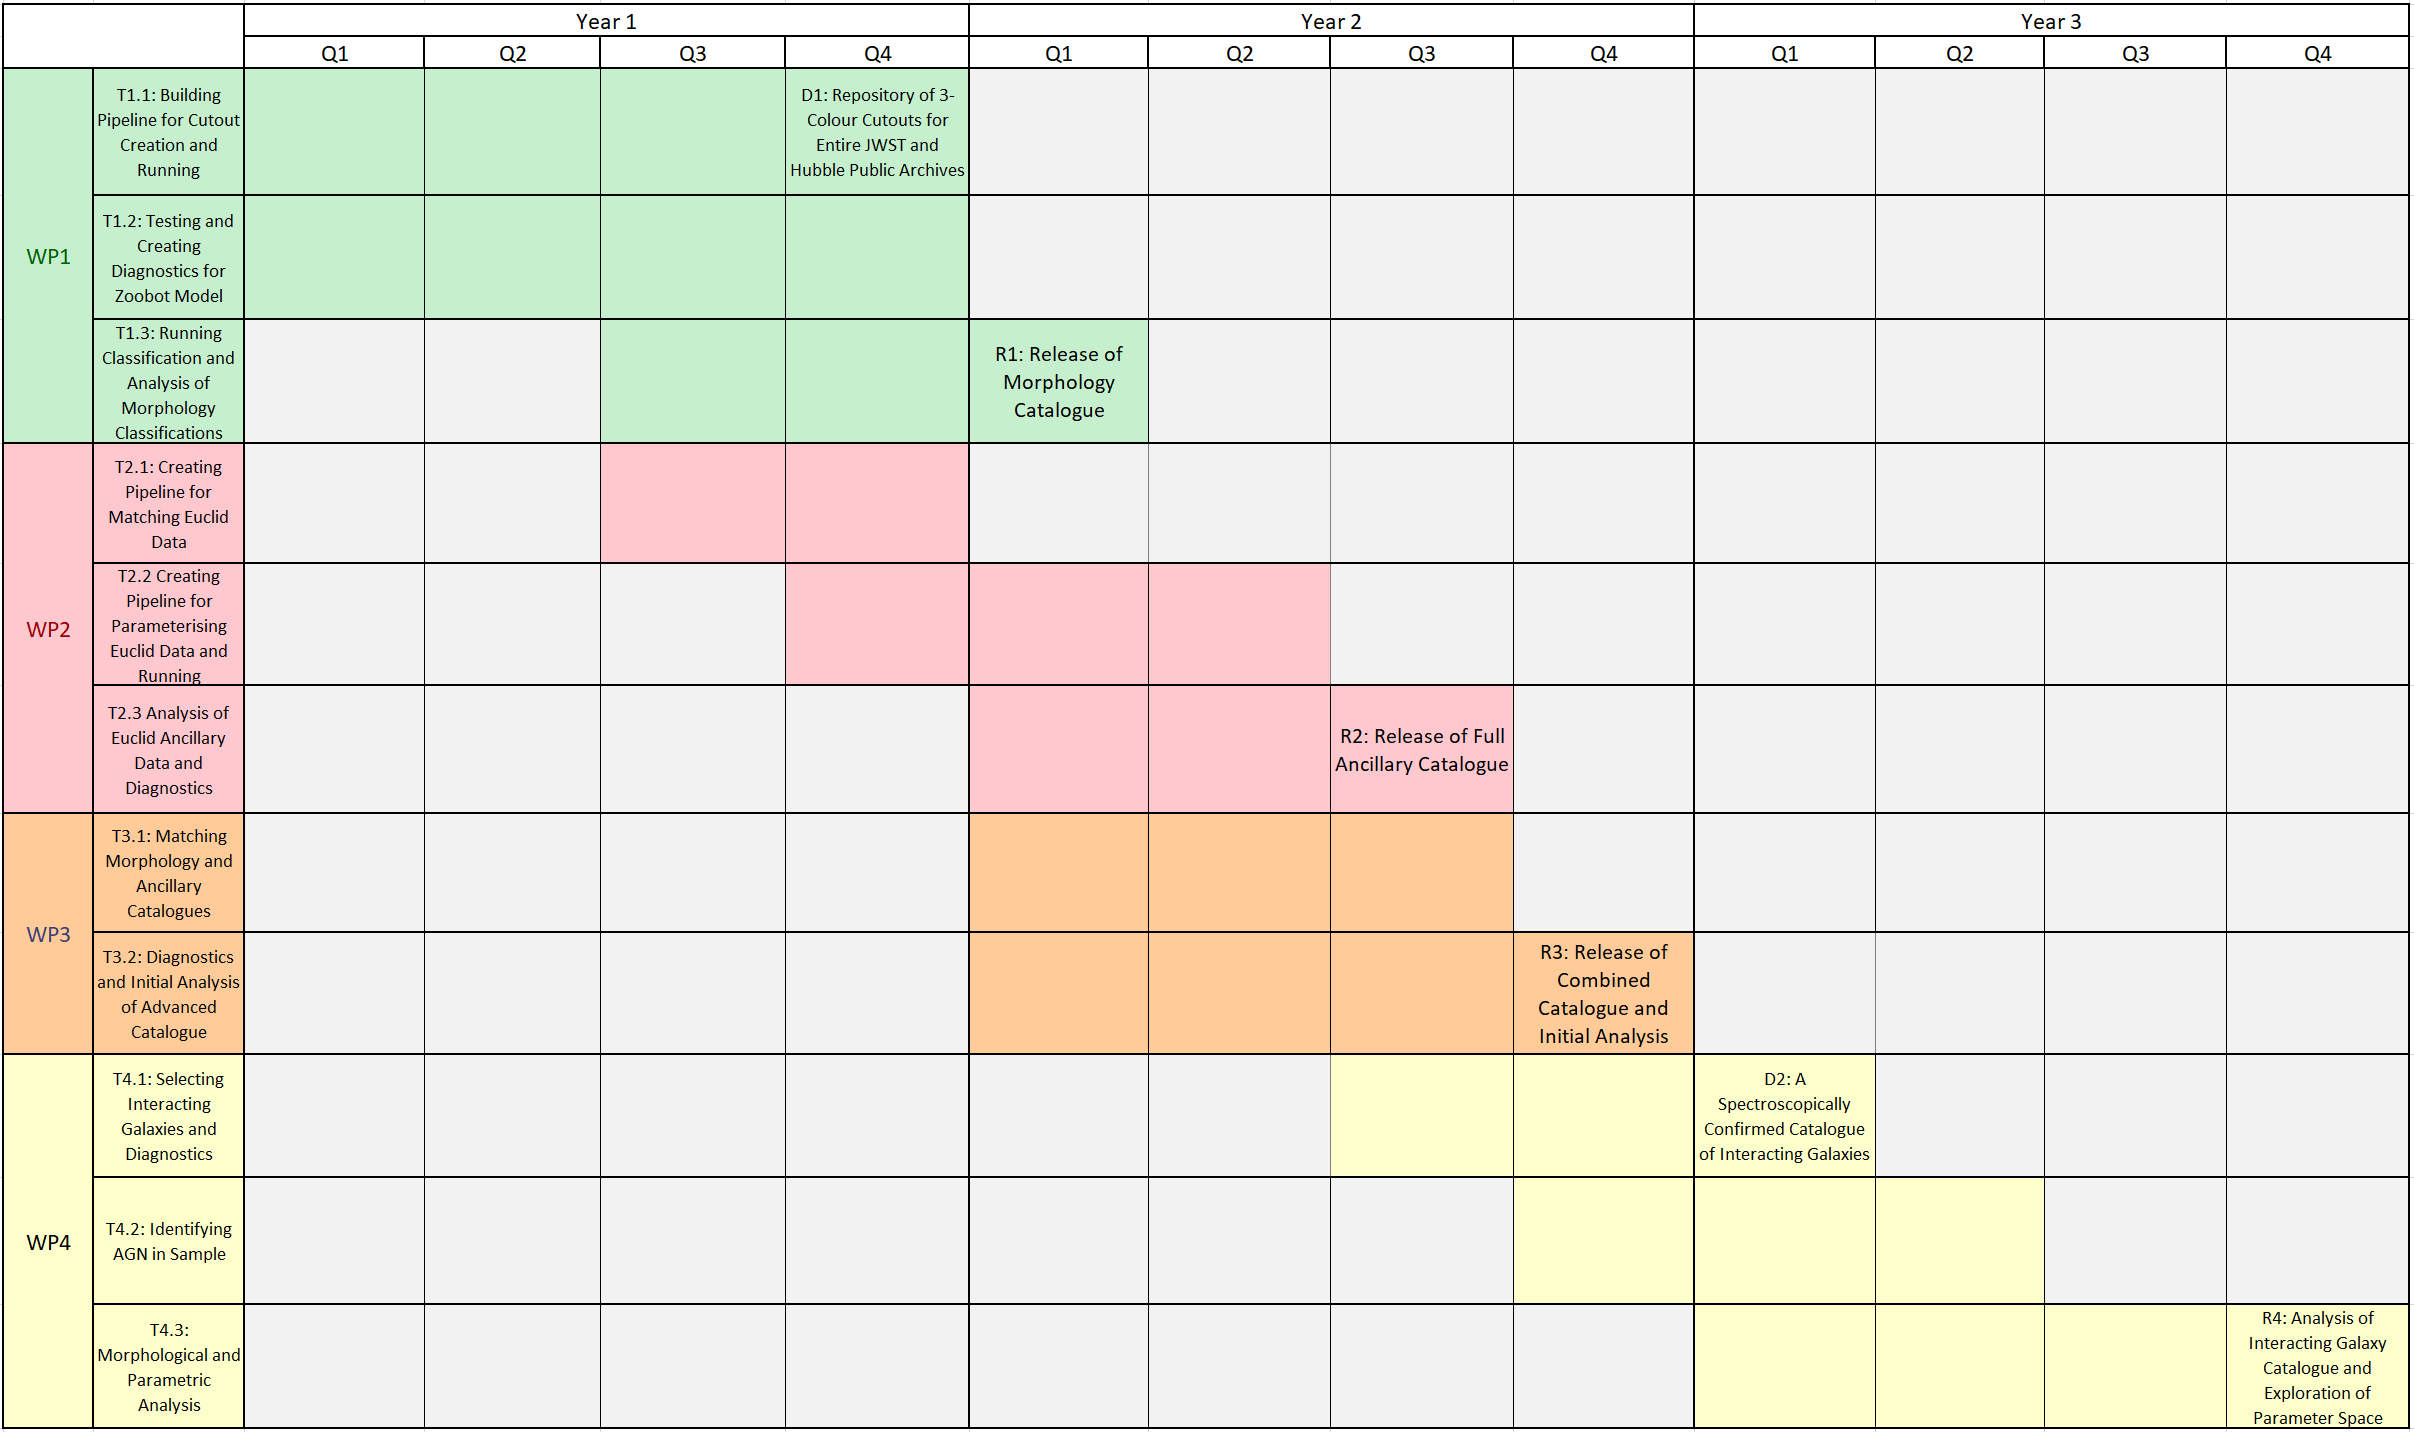
\includegraphics[width = 0.95\textwidth]{figures/draft-gantt-v2.png}
    \caption{GANTT chart of proposed project timeline. Includes workpackes (WP$N$), scientific results (R$N$) and deliverables (D$N$).}
    \label{fig:gantt-chart}
\end{figure}

% \noindent \textbf{WP1: Exploring the Archives for a Large Catalogue of Galaxy Morphologies} \\
% \noindent To create a catalogue of morphological classifications, the following tasks must be completed:
% \begin{enumerate}[itemsep=0pt, parsep=0pt, topsep=5pt]
%     \item A pipeline to create a cutout of every source to be classified must be built.
%     \item The pipeline must be run, creating the cutouts.
%     \item The classification model (\texttt{Zoobot}) must be tested and diagnosed.
%     \item The classification model must be run on all sources created.
% \end{enumerate}
% The outputs of these tasks will include the first deliverable of the project (D1): a repository of images of ever source in the \textit{Hubble} and JWST archives. This is an output of tasks 1. The first scientific result of this project will also come from this, with a paper defining the new morphological catalogue and  \\

% \noindent \textbf{WP2: An Ancillary Catalogue for 126 million+ Sources} \\
% \noindent Upon the completion of WP1, Euclid will have been operational for roughly a full year. By utilising existing SED analysis software, a catalogue of parametric data will be created. Specifically, this will be done using the EAzY and FAST softwares, providing calculations of many parameters of importance. Once this is produced, this will be combined with the morphology catalogue created in WP1. \\

% \noindent \textbf{WP3: Analysis of the Advanced Catalogue} \\
% With the full catalogue created, a census of a multitude of galaxy types can be conducted. The catalogue will be broken down into each different morphology available, and complete and incomplete data quantified. I will conduct initial analysis will be conducted on the data, such as quantifying the catalogues selection effects, completeness and accuracy. This will be achieved by comparing to existing catalogues such as COSMOS and existing large Galaxy Zoo catalogues to show that morphology proportions are reasonably consistent. I will also conduct an initial analysis relating star formation rates, stellar masses and nuclear activity different morphologies. \\

% \noindent \textbf{WP4: Exploring the Interplay of Galaxy Interaction and Nuclear Activity} \\
% In the final year of the project, to demonstrate the power of the new catalogue, I will investigate the specific interplay between galaxy interaction and nuclear activity. By selecting all interacting, merging or disturbed galaxies from such a large catalogue and using the measured Euclid ancillary data it will be possible to identify galaxies containing an active galactic nuclei and those which do not. With these identified, the parameters of each can be explored further and investigated.

\synergy
\vspace{-3mm}
As stated throughout this proposal, this project is directly related to multiple ESA missions. The two primary missions it will take advantage of is the development of the archives with ESA Datalabs and the new flagship mission Euclid. The archives, and the new infrastructure built around it, form a key cornerstone of this project. Without ESA Datalabs and the unique kind of access to archival data it provides, this project would not be possible. The second cornerstone of this project is Euclid. To date, no such all-sky spectroscopic survey to the scale of Euclid exists. Combining archival data with Euclids spectroscopy will lead to an advanced catalogue of a size yet seen in the field.

This project will also use the ESA-NASA mission JWST. The volume of available JWST archival data is now impossible to ignore and not utilise. This archival data is specifically available on ESA datalabs, and can be accessed by simple adaption of our pipelines, as they exist. The ancillary data JWST provides, as well as its unique spectroscopy and imaging of high redshift systems will allow us to create a more complete catalogue which accounts for this regime.

My previous experience with ESA Datalabs, \texttt{Zoobot} and utilising the ancillary data of the COSMOS catalogue put me in a unique position to create and analyse these new advanced catalogues. While building the pipelines to create cutouts, or conduct classifications, would certainly take time to build the fact that I have much of these pipelines ready for use will significantly streamline the ramp up of the project. From this project, I also hope to fully demonstrate the power of Euclid combined with that of ESA Datalabs and the archives. Giving a new dataset to the field which is unprecedented in scope.

\begin{multicols}{2}


\bibliographystyle{mnras}
\bibliography{references}


\end{multicols}

% \noindent \textbf{Creating Statistically Robust Galaxy Samples with ESA Datalabs} \\
% As shown in my first paper \citep{O'Ryan}, it is possible to create extremely large catalogues of different astrophysical objects even under very conservative conditions. In that project, we utilised the CNN \texttt{Zoobot} in conjunction with direct access to the \textt{Hubble} Science Archives via ESA Datalabs. The resultant catalogue of 21,926 interacting galaxies was the largest catalogue of interacting galaxies at the time of publication. However, in making such a catalogue (in such a short timeframe) certain sacrifices had to be made. First, there are multiple issues with identifying interacting galaxies by visualisation alone. Often contamination by close pairs (i.e. galaxies close together by projection effects on the sky, not actually interacting) outweight any interacting galaxies found. This collapse of purity often makes seemingly large, statistically robust, catalogues useless. Therefore, in this project we focused on interacting galaxies which specifically had tidal features; focusing the CNN on classifying them. This focuses the catalogue on a specific timeframe of interaction. The second sacrifice was that of purity over completeness. We used incredibly conservative classification criteria when defining an interacting galaxy - due to the problem of close pairs. This means that may real interacting galaxies will have been misidentified as non-interacting.

% However, what this project demonstrated was the capability of leveraging the archives to make the largest possible catalogues of astrophysical objects of interest to date. Not only did I find interacting galaxies with this approach, but also a whole host of other objects in the contamination of the final catalogue. Therefore, if given the opporunity, I would expand this project significantly. With further upgrades to \texttt{Zoobot} since I used it, it's accuracy for this task has dramatically improved. While I would focus on releasing a complete catalogue of interacting galaxies (and calculating that completeness) I would also release catalogues of many different kinds and morphologies of galaxies. There are many astrophysical objects which we only have a few dozen examples. By leveraging the archives, I would expand those catalogues by an order of magnitude - as I did for interacting galaxies.

% The key difference between the project I propose here and the internship I conducted is the shift in focus to analysis and followup. This project will be conducted at a time where Euclid will begin taking data, the James Webb Space Telescope (JWST) has already obtained a treasure trove of data and the development of ESA Datalabs is nearing its completion. Because of my experience with ESA Datalabs and the archives when their development was only just beginning, I m well suited to take advantage of these tools immediately and get quick returns on their deployment. The only barrier to me, currently, is that I am not in the Euclid consortium to take immediate access of the data. However, if this application progresses, I will begin the process of joining it so I can access and utilise their data. This will be paramount, as the second focus of this proposal is to begin anaylsis of the objects we find through the archives. This requires ancillary data. That ancillary data will come from Euclid, and the softwares described previously. The power of this combination is already becoming apparent, with the investigation of the \citet{O'Ryan} catalogue using the COSMOS field. This case study is explained in the next section, and then the full scope of this project revealed.
% \\
% \\
% \noindent \textbf{The Success of the COSMOS Catalogue and the Potential of Euclid} \\
% An example of value adding to the catalogues that will come out from the archives is that of comparing my \citet{O'Ryan} catalogue to the COSMOS catalogue. COSMOS is a catalogue of ancillary data. It contains the coordinates of over 1.7 million sources (the COSMOS2020 Classic catalogue does), as well as observed magnitudes and emissions from each. The true value then comes from the catalogue team applying the previously described softwares to their sources. This allows them to also publish, with the observations and source coordinates, estimates of photometric redshifts, estimates of stellar masses, star formation rates, etc. These can then be used to infer relations between the types of galaxies and their parameters.

% We conducted a matching between COSMOS and the \citet{O'Ryan} catalogue purely on source coordinates, and recovered 3,897 matches. We were also able to recover the secondary galaxies in each of these systems, giving us ancillary data to a total of 7,794 interacting galaxies. While this analysis is only just coming to its conclusion, the prelimary results are fascinating. By breaking down each system into a different stage of interaction, we had found direct links between that and the star formation rates observed in them. We are also relating the stages to AGN activity, finding activation begins to occur in a specific stage. These results are shown in figure \ref{fig:comsos_results}.

% \begin{figure}
%     \centering
%     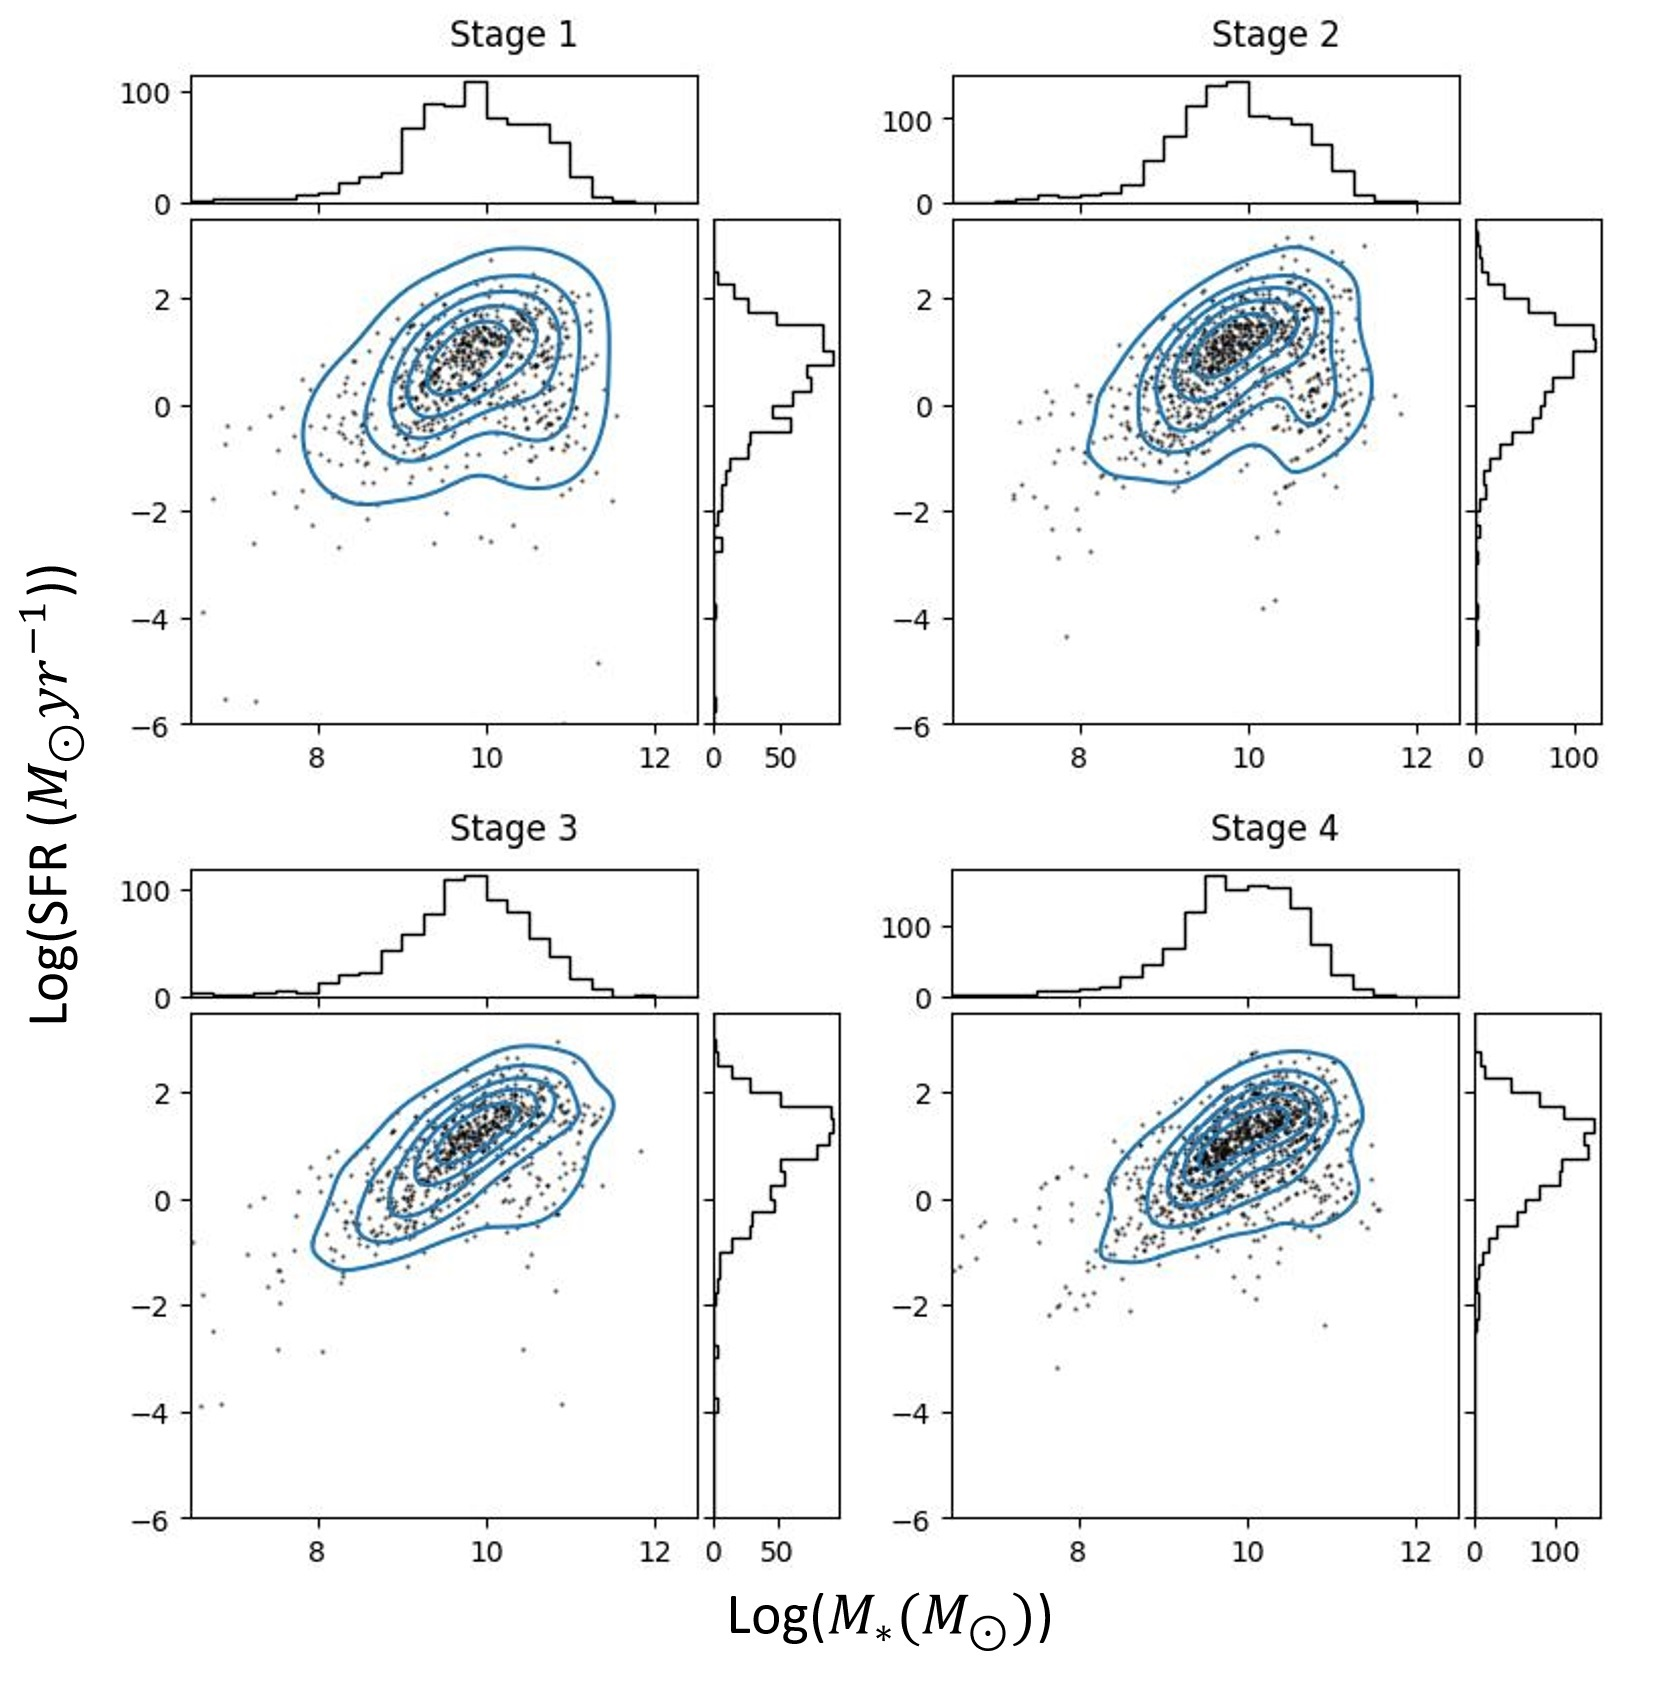
\includegraphics[width=\textwidth]{figures/stage-evol.jpg}
%     \caption{Initial results of combining the \citet{O'Ryan} catalogue with the ancillary data of the COSMOS catalogue. Each interaction has been broken up into different stages of interaction, and their stellar masses and star formation rates plotted. In stages 1 and 2, we see that there is a secondary population of high mass, lower star forming galaxies which disappears as we move into stages 3 and 4 of the interaction. This is shown best by the contours in each subplot, but can also be observed in the slope of the histograms. This is evidence of when a starburst may occur in interacting systems through an interaction, an important pieve of evidence we are missing in understanding the effects of interaction on the galactic population.}
%     \label{fig:cosmos-label}
% \end{figure}

% Now, these discoveries and inferences are coming from a fifth of the interacting galaxies in the \citet{O'Ryan} catalogue. This is simply a fact of those galaxies which overlap with the COSMOS field. However, Euclid will allow us to bring a completely new scale to this approach. While the observing area of the COSMOS field is relatively small (approximately $3^{\circ} \times 3^{\circ}$) Euclid will be an all sky survey mission. Not only could the entirety of the \citet{O'Ryan} catalogue be covered by Euclid, and ancillary data created for it, but any objects of astrophysical interest throughout other catalogues we find will have ancillary data available.

% Thus, this project will aim to combine the approaches of the Galaxy Zoo and COSMOS collaborations. The specific relating of galactic parameters (stellar masses, sizes, environment, etc) to physical processes (star formation, nuclear ignition, bar formation, etc) is poorly understood and constrained. The connection between such parameters and morphology is a further complication. Often, it is impossible to directly investigate both morphology and parameterisation simultaneously due to a lack of overlap between the data. In this project, we will be creating both sets of data for every object in the \texttt{Hubble} archives which is also overlapped by Euclid. Before doing any analysis, I predict the usefulness of these catalogues will be huge in the community. For reference, the first Galaxy Zoo paper \citep{lintott_08} has 806 citations while the initial COSMOS catalogue data release has 695 citations. Therefore, the potential impact of releasing a combined catalogue, before we conduct any fundamental analysis, of morphological and galactic parameterisation is colossal.
% \\
% \\
% \noindent \textbf{Aside: Parameterisation of Interacting Galaxies} \\
% \noindent While the focus of this project will be on creating and analysing the results of statistically robust, ancillary complete catalogues of all kinds of galaxies a special focus will be given to interacting galaxies. My PhD project has been focused on constraining galaxy interaction by directly comparing simulations to observations. The aim has been to parameterise the galaxies involved in the interaction and relate those parameters to the tidal features that form in the interaction. Initial results found by comparing to those from Galaxy Zoo: Mergers project will soon be pulished, showing the viability of this approach. The approach utilises an efficient N-body interaction modeller with Markov-Chain Monte Carlo methods to fully explore a pre-defined parameter space and show the parameter values that have the highest probability of forming those tidal features. The limitation of this, in my PhD, was that this approach was only applied to a sample of sixty interacting galaxies: hardly a statistically significant sample. 

% Using the catalogues generated here, interacting galaxies will be identified (similar to in \citet{O'Ryan}). However, using Euclid they will also be spectroscopically confirmed. This will give us a sample of high purity and completeness, eradicating the problem of close pairs entirely. I will then apply the methods developed in my PhD to this sample, and demonstrate an initial use of the catalogues we are creating. I will fully statistically constrain which areas of parameter space of interaction lead to the formation of tidal features for the full population of interacting galaxies. As the work developing this code has been completed in my PhD, I will simply have to apply it to the resulting catalogues of this project to investigate this. 

% \vspace{-3mm}
% \describearchival
% \vspace{-3mm}
% \noindent\textbf{Project Timeline \& Project Results} \\
% \noindent The timeline described in this section assumes a project timescale of 3 years and is laid out as shown in Fig \ref{fig:gantt-chart}. Each specific part of the project has been broken down into different work packages (WP) and then broken down into tasks to be completed. The definition of of each work package, and the tasks involved is explained below.

% \noindent \textbf{WP 1: Building the Classification Pipeline, Training and Creating a Morphological Catalogue} In order to classify the morphology of greater than 126 millions sources, a robust pipeline will need to be built. This pipeline must be able to: create reasonable source cutouts in a general way, be able to identify bad cutouts, feed them into a trained classifier and be fully diagnostically checked before running on the full sample and classifying every source. In my internship at ESAC, this part was the bulk of the project. I, therefore, will be putting at least 4 quarters into this part. This work package will also include the writing up of a large data release as well as a breakdown of objects of interest found. This resultant paper will be analogous to \citet{O'Ryan}.

% \noindent \textbf{WP 2: Analysing Morphological Classifications} Once the pipeline has been completed, and run upon all sources, excellent analysis can then be conducted involving the specific morphologies. What will be of intense interest to myself will be building a link here between the existence of morphological structures and environment. I will also aim to cross-match any sources found here with existing catalogues of ancillary data to link in photometric parameterisations. Therefore, I aim to build links, specifically, between environmental density, the formation of galactic structures (such as bars or spirals) and photometric galactic parameters (such as star formation rates and stellar mass).

% \noindent \textbf{WP 3: Analysing Euclid Data and Creating Photometric Parameterisation} By the time the previous two WPs have been completed, the first few data releases from Euclid should be publicly available (or, at least, available within the consortium). I will spend the time here gauging the work required to build the ancillary catalogue to go with the morphological one. I will mess around with Euclid data, and investigate what reductions must be done with it. I will then utilise EAZY, LePhare and FAST to calculate photometric galaxy parameters of any overlapping data. I will then release this ancillary catalogue to the community. Assuming that there is sufficient overlap to build a statistically significant sample, I will investigate any links between environment, morphology and photometric parameters over this wider sample. At this stage, I will also begin to specifically select out interacting galaxies from the sample for WP 4.

% \noindent \textbf{WP 4: Use Case of Catalogue: Interacting Galaxies} In the final WP, I shall conduct a deep dive on using the new catalogue of objects specifically with regard to interacting galaxy. Using this large sample of photometrically confirmed interacting galaxies, I will investigate relations between the photometric parameters, interaction stage, the tidal features formed, nuclear activity and star formation rate enhancement. I will also apply my own algorithm to this sample, and explore the full parameter space of interaction and find which parameters lead to specific tidal features.
% \\
% \\
% The first year of this project will primarily be focused on developing the code to extract excellent cutouts of all sources in the \texttt{Hubble} source catalogue. While I currently have the code to generate these cutouts from my internship, some refinements must be made. Specifically, the size of the cutout must be based upon the size of the source within it. This will ensure the source is fully resolved in the cutout; an issue discovered when keeping a fixed cutout size in the \citet{O'Ryan} catalogue. This time will also be used to test the accuracy of \texttt{Zoobot} through different \texttt{Hubble} filters and instruments. For these tests I will need to create training sets of different galaxies with full descriptions from Galaxy Zoo.

% Once the code is created and tested, it will be run on the entire \texttt{Hubble} archives across all filters and instruments. The classification will take some time. From the creation of the \citet{O'Ryan} catalogue, 92 million sources took approximately one month to classify. As we add further source catalogues or instruments into our pipeline, the classification process itself may take more than this. We therefore schedule in 2.5 months for this process. As this process continues, I will shift my focus to the secondary goals of this project. I will begin to investigate Euclid data and get acquainted with it. I will focus my attention on interacting galaxies and further constraining the \citet{O'Ryan} catalogue. I will also have access to the results as they come in, allowing me to investigate the results and make some preliminary investigations into what we might find. I will also begin building the pipeline that will utilise the ancillary data to compute each galaxies parameterisation.

% Finally, in the third year of this project, I will conduct the key analysis of the full catalogue we create. I will present an initial review of the parameter space we have covered as well as the limitations of the catalogue. I will the conduct an investigation into the different types of galaxies vs the parameterisations we have made. I will pick out the interacting galaxies for an example paper of how to use the catalogue, and do a in-depth exploration of their parameter space. To finalise the project, I will conduct my own analysis of the new interacting galaxy sample and apply the software developed in my PhD to completely match the underlying parameter space to tidal features that form. \\

%%%% Rewrite above, but put it in terms of Work Packages with specific goals. 
% Work Package 1: Building the pipeline that will conduct the classifications of the objects.
% Work package 2: Analysing the resultant data from all objects in HSC. Also diagnosing model completeness, purity, etc.
% Work Package 3: Combining with Ancillary data from Euclid. This includes checking Euclid data and applying photometric algorithms.
% Work Package 4: Deep dive on interacting galaxies and conducitng their full parameterisation.

% \noindent\textbf{Expected Science Results} \\
% \noindent Here, we describe the specific scientific outputs expected from each WP. Currently, they are simply the names of the papers expected, but can be expanded upon further on request. From the four work packages, I anticipate that there will be five scientific publications. The titles of these will be:

% \begin{enumerate}[itemsep=0pt, parsep=0pt, topsep=0pt]
%     \item \textbf{WP1}: A Complete Sample of Interacting Galaxies: An Initial Exploration
%     \item \textbf{WP1}: A Morphological Catalogue of 126 Million Sources from the Hubble Source Catalogue
%     \item \textbf{WP2}: Combining Morphology and Parameterisation: A Morphology Catalogue Matched to COSMOS
%     \item \textbf{WP3}: Linking Morphology and Euclid: A Catalogue of N Galaxies with full Morphological and Ancillary
%     \item \textbf{WP3} Leveraging Parameterisation: A Statistical Study Linking Galaxy Parameters to Galaxy Types
%     \item \textbf{WP4} Exploring the Interacting Galaxy Population: Linking Underlying Parameters to Feature Formation
% \end{enumerate}

% \noindent On top of these, I will also aim to publish two further works on what we find in the archives. These will be relatively short, low hanging fruit papers which provide coordinates and classifications of rare astrophysical objects to the community:
% \begin{enumerate}[itemsep=0pt, parsep=0pt, topsep=0pt]
%     \item \textbf{WP1.1}: The Gems of the Archives: Release of a Catalogue of Rare Galaxy Types from the \texttt{Hubble} Archives
%     \item \textbf{WP4.1}: Directly Investigating Interaction: Exploring the Underlying Parameter Space of a Statistically Robust Sample of Interacting Galaxies
% \end{enumerate}

% See how I did this in the FlatIron proposal. And then we've just got to make the damn thing fit. 
% Fit, re-read and then make sure we have everything!
% \noindent \textbf{References}\\
% {}

\end{document}